%&../../.preamble
\endofdump
\usetikzlibrary{patterns}
\begin{document}
\begin{enumerate}
	\item Quando eseguiamo un esame clinico per accertare la presenza di una certa patologia, il test può risultare positivo (abbiamo la patologia) oppure negativo. L'esame può commettere errore, ad esempio, il test può risultare positivo ma noi non abbiamo la patologia (si parla di falso positivo). La probabilità che il test sia negativo e noi non abbiamo la patologia è chiamata specificità, mentre, la probabilità che il test sia positivo quando effettivamente abbiamo la patologia è chiamata sensibilità. Infine la probabilità di avere una certa patologia è chiamata prevalenza. Vi siete sottoposti al test per accertare la presenza di HIV. Nella popolazione la prevalenza di HIV è di 6.1 casi su $1 e+05$. Il test ELISA ha una sensibilità pari a 0.999 , mentre i falsi positivi sono pari a $7 e-04 \%$.
	      \begin{enumerate}
		      \item Definire lo spazio probabilizzabile che serve per descrive questo esperimento.
            \vskip3mm 
            \begin{center}
                          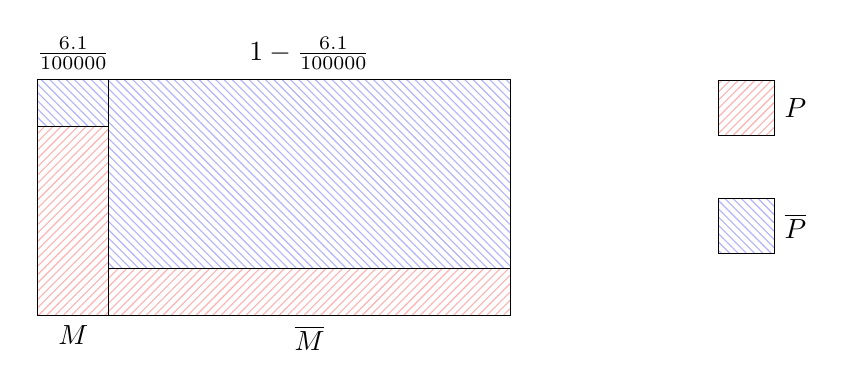
\begin{tikzpicture}[scale = 3]
                            \draw [pattern = north east lines, pattern color = red!30](0,0)--++(0,0.8)--++(0.3,0)--++(0,-0.6)--(2,0.2)--(2,0)--cycle;
                          \draw [pattern = north west lines, , pattern color = blue!30](0,1)--(0,0.8)--++(0.3,0)--++(0,-0.6)--(2,0.2)--(2,1)--cycle;
                          \node [anchor = south] at (0.15,1) {$ \frac{6.1}{100000} $};
                          \node [anchor = north] at (0.15,0) {$ M $};
                          \node [anchor = south] at (1.15,1) {$ 1-\frac{6.1}{100000} $};
                          \node [anchor = north] at (1.15,0) {$ \overline{M} $};
                          \node (a)[anchor = north, pattern = north east lines, draw, inner sep = 10pt,pattern color = red!30]at (3,1) {};
                          \node [anchor = west] at (a.east) {$ P $};
                          \node (a)[anchor = north, pattern = north west lines, draw, inner sep = 10pt,pattern color = blue!30]at (3,0.5) {};
                          \node [anchor = west] at (a.east) {$ \overline{P} $};
                          \draw (0,0)rectangle(2,1);
                          \draw (0.3, 1)--(0.3, 0);
                          \draw (0.3, 1)--(0.3, 0);
                          \draw (0, 0.8)--(0.3, 0.8);
                        \end{tikzpicture} 
            \end{center}
            Pongo $ \omega  = \left\{\left(P,M\right), \left(\overline{P}, M\right), \left(\overline{M}, P\right), \left(\overline{M}, \overline{P}\right)\right\} $. La tribù può essere l'insieme delle parti di $ \omega  $
		      \item Calcolare la probabilità che il test risulti positivo.
            \vskip3mm 
            \begin{align*}
              \Pr \left(\right)
            \end{align*}
		      \item Calcolare la probabilità che siccome il test è positivo voi abbiate realmente l'HIV.
		      \item La probabilità che una persona con l'HIV sia un maschio è 0.976 , mentre la probabilità che una persona che non ha l'HIV sia un maschio è 0.5. Inoltre la specificità e la sensibilità del test non dipende dal genere della persona. Alla luce di questa informazione, ricalcolate la probabilità che, dato che il test è positivo, voi abbiate realmente l'HIV.
	      \end{enumerate}
	\item Sia $Z=(X, Y)$ una variabile aleatoria doppia con funzione di probabilità:
	      \[
		      f_Z(z)=f_{X, Y}(x, y)=\frac{\lambda^x x^y \exp (-(\lambda+x))}{x ! y !}
	      \]
	      con $x, y \in\{\mathbb{N} \cup 0\}$ e $\lambda>0$. Calcolare
	      \begin{enumerate}
		      \item  la funzione di probabilità (marginale) della variabile aleatoria $X$;
		      \item fissato $\lambda=3$, il valore atteso e la varianza della variabile aleatoria $X$;
		      \item la funzione di probabilità (condizionale) della variabile aleatoria $Y \mid X=3$.
		      \item il valore atteso e la varianza della variabile aleatoria $Y \mid X=3$;
		            i
	      \end{enumerate}
	\item Un pronto soccorso ha in servizio 20 ambulanze. Per ragioni di manutenzione non in tutti i giorni tutte le ambulanze sono disponibili. In 8 giorni si sono avute disponibili un numero di ambulanze pari a:
	      \[
		      \begin{array}{llllllll}
			      1 & 1 & 1 & 1 & 0 & 1 & 0 & 2
		      \end{array}
	      \]
	      \begin{enumerate}
		      \item Si proponga una famiglia parametrica adatta a descrivere il fenomeno oggetto di studio;
		      \item Si calcoli la stima con il metodo dei momenti dei parametri coinvolti nella famiglia;
		      \item Si calcoli una stima intervallare di livello 0.95 per i parametri coinvolti;
		      \item Si calcoli la stima del valore medio di ambulanze disponibili in un giorno (si usi il metodo del plug-in);
		      \item Si calcoli una stima intervallare di livello 0.95 per il valore medio di ambulanze disponibili.
	      \end{enumerate}
\end{enumerate}
\end{document}
